\documentclass[border=4pt]{standalone}
\usepackage{amsmath,amssymb,amsfonts}
\usepackage{xcolor,colortbl,array,booktabs,multirow}
\usepackage{tikz}
\usepackage{pgfplots}
\pgfplotsset{compat=1.16}
\usetikzlibrary{arrows, automata, backgrounds, calendar, chains, decorations,
    matrix, mindmap, patterns, petri, positioning, shadows, shapes.geometric,
    trees, shapes, decorations.pathreplacing, calc, tikzmark, arrows.meta,
    intersections, fit, graphs, quotes, angles, decorations.markings}
\newcommand{\st}{\text{ s.t. }}
\newcommand{\x}{\mathbf{x}}
\renewcommand{\b}{\mathbf{b}}
\renewcommand{\c}{\mathbf{c}}
\newcommand{\A}{\mathbf{A}}
\newcommand{\y}{\mathbf{y}}
\newcommand{\z}{\mathbf{z}}
\newcommand{\R}{\mathbb{R}}
\newcommand{\RR}{\mathbb{R}}
\newcommand{\Z}{\mathbb{Z}}
\newcommand{\ZZ}{\mathbb{Z}}
\newcommand{\npcomplete}{NP-complete}
\providecommand{\true}{\text{TRUE}}
\providecommand{\false}{\text{FALSE}}
\tikzset{vertex/.style={circle,fill=black!25,minimum size=20pt,inner sep=0pt},
    edge/.style={draw,thick,-},weight/.style={font=\small},
    selected vertex/.style={vertex, fill=red!24},
    selected edge/.style={draw,line width=2pt,-,red!50},
    ignored edge/.style={draw,line width=2pt,-,black!20}}
\newcommand{\vect}{\vec}
\providecommand{\ds}{\displaystyle}
\providecommand{\longvect}{\overrightarrow}
\usepackage[normalem]{ulem}
\definecolor{ocre}{RGB}{243,102,25}
\providecommand{\leftB}{\left[}
\providecommand{\rightB}{\right]}
\tikzset{directed/.style={postaction={decorate,decoration={markings,mark=at position .65 with {\arrow{>}}}}},
    directed1/.style={postaction={decorate,decoration={markings,mark=at position .65 with {\arrow{>}}}}}}
\begin{document}
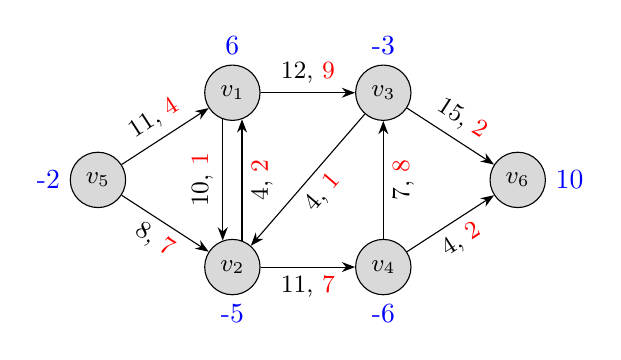
\begin{tikzpicture}[
      mycircle/.style={
         circle,
         draw=black,
         fill=gray,
         fill opacity = 0.3,
         text opacity=1,
         inner sep=0pt,
         minimum size=20pt,
         font=\small},
         startcircle/.style={
         circle,
         draw=black,
         fill=green,
         fill opacity = 0.3,
         text opacity=1,
         inner sep=0pt,
         minimum size=20pt,
         font=\small},
         endcircle/.style={
         circle,
         draw=black,
         fill=red,
         fill opacity = 0.3,
         text opacity=1,
         inner sep=0pt,
         minimum size=20pt,
         font=\small},
      myarrow/.style={-Stealth},
      node distance=0.6cm and 1.2cm
      ]
      \node[mycircle, label = {left: {\color{blue}-2}}] (c1) {$v_5$};
      \node[mycircle,below right=of c1, label = {below: {\color{blue}-5}}] (c2) {$v_2$};
      \node[mycircle,right=of c2,label = {below: {\color{blue}-6}}] (c3) {$v_4$};
      \node[mycircle,above right=of c1, label = {above: {\color{blue}6}}] (c4) {$v_1$};
      \node[mycircle,right=of c4, label = {above: {\color{blue}-3}}] (c5) {$v_3$};
      \node[mycircle,below right=of c5, label = {right: {\color{blue}10}}] (c6) {$v_6$};
      

    \foreach \i/\j/\txt/\txtr/\p in {% start node/end node/text/position
      c1/c2/8/7/below,
      c1/c4/11/4/above,
      c2/c3/11/7/below,
      c3/c6/4/2/below,
      c4/c5/12/9/above,
      c5/c6/15/2/above,
      c5/c2/4/1/below,
      c3/c5/7/8/below,
      c2.70/c4.290/4/2/below}
       \draw [myarrow] (\i) -- node[sloped,font=\small,\p] {\txt, {\color{red} \txtr}} (\j);

% Commented-out foreach (all list entries were removed)
%\foreach \i/\txt/\p in {%
%      c1/8/left,
%      c2/11/above,
%      c3/2/below,
%      c4/9/above,
%      c5/2/above,
%      c6/1/below}
%\node[\p] (\i) {\txt};

     % draw this outside loop to get proper orientation of 10
     \draw [myarrow] (c4.250) -- node[sloped,font=\small,above,rotate=180] {10, {\color{red} 1}} (c2.110);
    \end{tikzpicture}
\end{document}
